\chapter{Optimization with non-stationary demand curve}
\label{chap:ns_demand}

\section{Environment behavior}
\label{sec:ns_demand_env}

\subsection{Overview}

By using the \textbf{non-stationarity} assumption we are taking into consideration that the demand curve could be subject to changes over time and isn't necessarily fixed as we have seen in other steps.

There are 2 main types of \textit{non-stationary behaviors}:
\begin{itemize}
    \item \textbf{Abrupt changes}: where it's possible to identify different phases with different phase-wise stationary demand curves.
    \item \textbf{Smooth changes}: where the demand curve changes over time in a continuous manner.
\end{itemize}

As per specifications, we will only consider \textbf{abrupt changes} in the scope of our project.

\subsection{Abrupt changes}

Abrupt changes are usually experienced when an important event strikes the market \textit{(e.g. a new product that shifts the interests of the users is released or an historical event shapes the opionion of people)}; change isn't necessarily bad, however, it may impact negatively the prediction of learners that were created with a static environment in mind.

Neither UCB nor TS account for abrupt changes since it's almost impossible for them to try a superarm that was deemed as \textit{unoptimal} over the past iterations (while it might have become optimal after an abrupt change), therefore we expect to see a significant reward drop from them after an abrupt change.

In the early stages of the project we noticed that the simulation that we created wasn't really fit to dinamically include abrupt changes in the environment, therefore great effort was spent in completely reworking the interface for the simulation from the ground-up.
Besides collateral improvements in reproducibility, results collection and user-friendliness, the new simulation allowed for an \textit{incremental simulation unfolding}, this meant that we were now able to simulate \textit{n} days, change the environment and simulate another \textit{n} days.
This particular feature revealed itself as fundamental for the upcoming challenges.

\section{Algorithms}
\label{sec:ns_demand_alg}

There are 2 main approaches to deal with a non-stationary environment

\begin{itemize}
    \item \textbf{Sliding window}: only consider the last $\tau$ samples for predictions.
    \item \textbf{Change detection}: detect when a change has happened and adapt accordingly.
\end{itemize}

It's clear that sliding window approaches are more fit for smooth changes while change detection approaches work better with abrupt changes, however it's important to note that both approaches can be utilized to deal with any \textit{non-stationary} scenario.

\subsection{Sliding window for TS and UCB}

\begin{itemize}
    \item \textbf{SW-GPTS} only differs in the gaussian process update since the older samples are progressively removed from the estimation as time goes on.
    \item \textbf{SW-GPUCB} also differs in the confidence bound formulation and the new arm choice:
        \begin{displaymath}
            a_t =
            \begin{cases}
                a_{\overline{t}} & \text{if} ~ \exists \overline{t} ~ | ~ n_{a_{\overline{t}}}(t-1, \tau) = 0 \\
                arg\max_{a \in A} \left\{ \mu_{t-1, \tau} + \delta \sigma_{t-1, \tau} \right\} & \text{otherwise}
            \end{cases}
        \end{displaymath}
\end{itemize}

\subsection{Change detection}

We used a reward-based algorithm as a change detection algorithm, it works by comparing the last $k$ rewards with the newest $k$ rewards ($k=4$ by default) and if the difference between their means exceedes a certain threshold $\omega$ ($\omega=1000$ by default) the learner is \textbf{reset} and is therefore able to learn a new optimal superarm from scratch.

Formally:
\begin{displaymath}
    \text{RESET learner if} ~ t \geq 2k ~ \land \sum_{i=t-2k}^{t-k} r_i -\sum_{i=t-k+1}^t r_i > \omega
\end{displaymath}

{\scriptsize N.B. there is an offset of 1 in the representation of t between theory and code}

\section{Results}
\label{sec:ns_demand_res}

Average reward and regret for the base learner

\begin{center}
    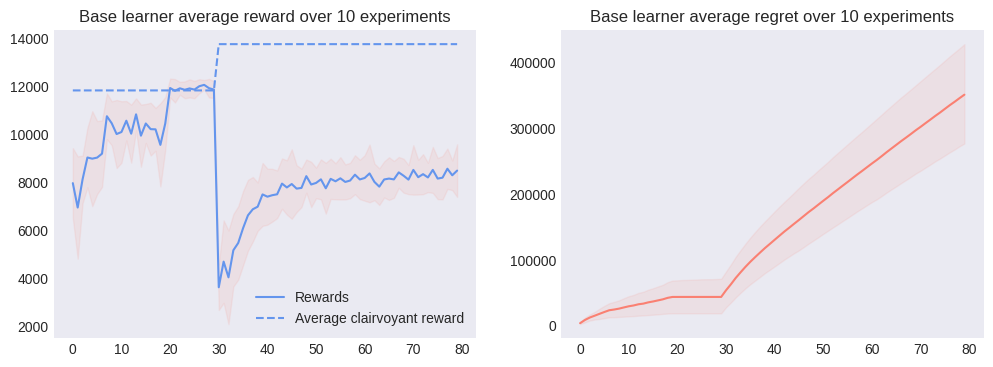
\includegraphics[scale=0.5]{img/Graphs/non_stationary/image1.png}
\end{center}

\clearpage % Aesthetic

Average reward and regret for the sliding window learner

\begin{center}
    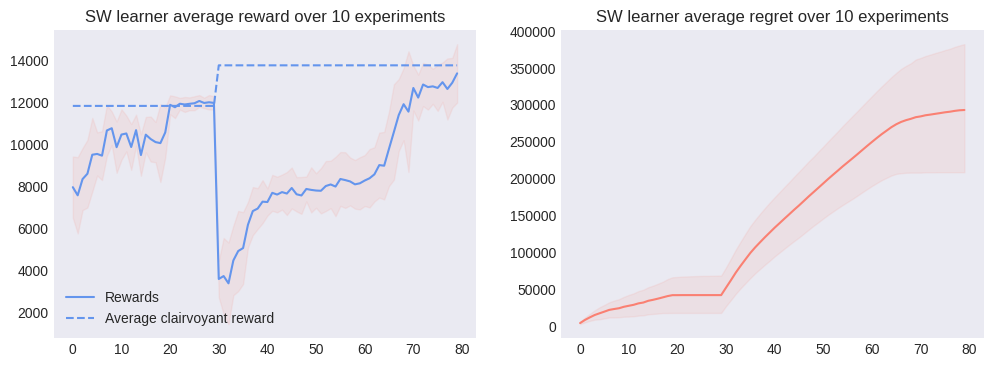
\includegraphics[scale=0.5]{img/Graphs/non_stationary/image2.png}
\end{center}

Average reward and regret for the change detection learner

\begin{center}
    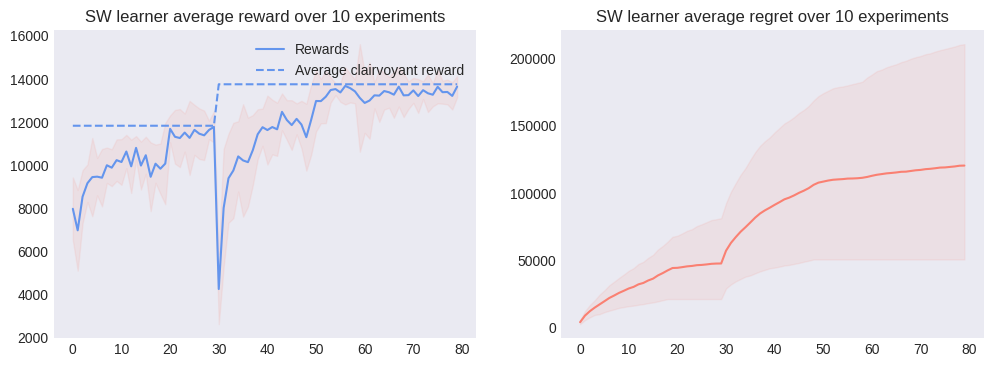
\includegraphics[scale=0.5]{img/Graphs/non_stationary/image3.png}
\end{center}

Reward and regret comparison

\begin{center}
    \hspace*{-3em}
    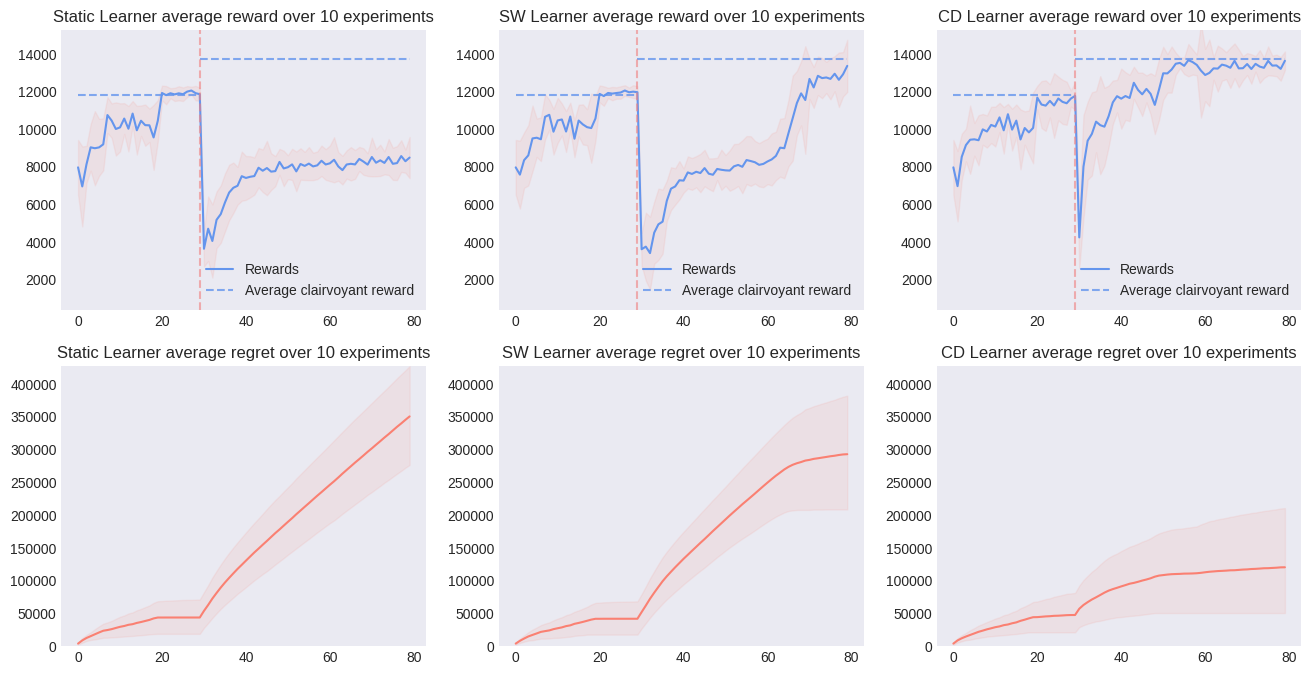
\includegraphics[scale=0.5]{img/Graphs/non_stationary/image4.png}
\end{center}

\clearpage % Aesthetic

All tests are done using the \texttt{example\_environment} with default values, \textit{population mean} of 1000, \textit{variance} of 10 and 20 \textit{budget steps}; while only UCB algorithms were evaluated and only one breakpoint was placed after 30 days.

\subsection{Conclusions}

From the results it's quite clear that the change detection algorithm is by far the best one in this specific scenario, while it's interesting to see that the sliding window approach it's slower to stabilize (due to the fact that the samples from the old environment must completely exit the window to not be considered) and the base learner approach isn't able to adapt, as expected.

Generalizing, we can say that if the number of breakpoints $m$ is small enough with respect to the time horizon $T$ to the power of $\alpha$ we have that the regret is of the order $O\left( \vert A \vert T^{\frac{1+\alpha}{2}} \right)$.

Average results over 10 runs at time horizon $T = 80$:

\begin{table}[h]
    \center
    \begin{tabular}{|c|cc|c|}
    \hline \hline
        \cellcolor{blue!25} & Reward 	& Regret	& Deviation \\
    \cline{2-4}
        \cellcolor{blue!25} & $\mu$		& $\mu$		& $\sigma$	\\
    \hline \hline
        Base learner		& 7717.40	& 376073.10	& 877.73	\\
    \hline
        Sliding window		& 12571.80	& 271383.60	& 908.26	\\
    \hline
        Change detection	& 13452.30	& 126329.10	& 684.53	\\
    \hline \hline
    \end{tabular}
\end{table}
